\documentclass[a4paper,11pt]{scrartcl}

\usepackage[margin=1in]{geometry}
\usepackage[scaled]{helvet}
\usepackage[T1]{fontenc}
\usepackage[utf8]{inputenc}
\usepackage{amsmath}
\usepackage{mathptmx}
\usepackage{courier}
\usepackage{graphicx}
\usepackage{ulem}
\usepackage{bookmark}
\usepackage{paralist}
\usepackage{ngerman}
\usepackage{fancyhdr}
\usepackage{float}
\usepackage{array}
\usepackage{lipsum}


\graphicspath{ {../img/} }
\renewcommand\familydefault{\sfdefault}




\pagestyle{fancy}
\fancyhf{}
\renewcommand{\headrulewidth}{0pt}
\fancyfoot[C]{
\includegraphics[width=\textwidth]{Polygon_gruen}\\ \thepage}


\rhead{
\includegraphics[width=\textwidth]{LogoHeader}}
\setlength\headheight{30pt}
\setlength\footskip{15pt}

\begin{document}
\renewcommand*{\arraystretch}{1.2}
\pagenumbering{gobble}
\begin{titlepage}
    \begin{center}
        \vspace*{1cm}\Huge
        \textbf{Softwarearchitektur}\par
        \vspace{0.5cm}\LARGE        
        Software Engineering II\par           
        \vspace{2cm}
        
\includegraphics[width=0.5\textwidth]{OptimaLogo_long}\par   
        \vspace{1cm}
        \textbf{Projekttitel: BonoboBoard}\par        
        \vfill\Large   
        Jakob Hutschenreiter (1419081)\\Jiesen Wang (9839152)\\Nick Kramer (3122448)\\Patrick Küsters (2598689)\\Peter Moritz Hinkel (2783930)\par
        %\vspace{2cm}  
        %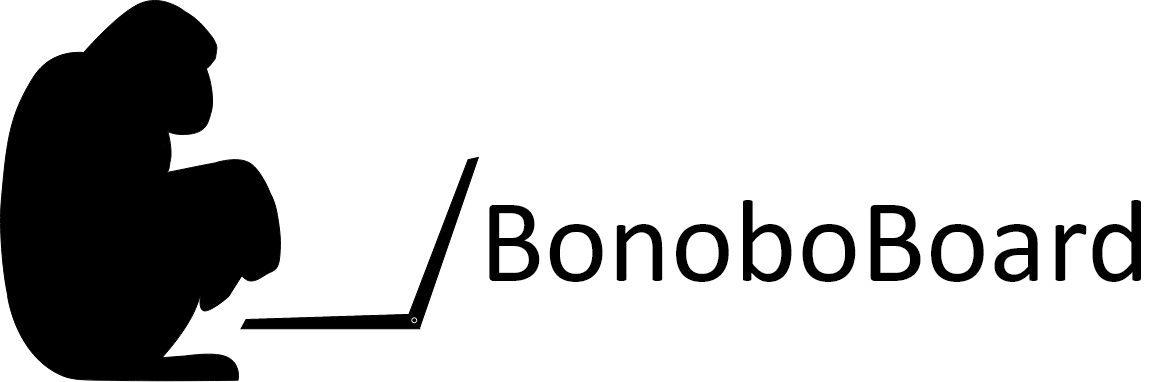
\includegraphics[width=0.5\textwidth]{Bonobo_Logo}\par        
        \vspace{2cm}
        DHBW Mannheim\\
        \today     
    \end{center}
\end{titlepage}

\section*{Änderungshistorie}
\begin{table}[h]
	\begin{tabular}{@{} p{20mm} p{25mm} p{35mm} p{75mm}}
		\textbf{Revision} & \textbf{Datum} & \textbf{Autor(en)} & \textbf{Beschreibung}\\
		1.0 & 22.02.2022 & NK|PK|JW|PH|JH & A: 1, 2, 3\\
	\end{tabular}
\end{table}
\noindent
Abkürzungen: Hinzugefügt/Added (A), Änderung/Changed (C), Löschung/Deleted (D)
\vspace{2cm}
\tableofcontents
\newpage
\pagenumbering{arabic}

		%------------------------------------------------------------
		%-----  -----  ----- Begin actual content -----  -----  -----
		%------------------------------------------------------------



\section{Einleitung}
Dieses Dokument befasst sich mit der Softwarearchitektur des Projekts "`BonoboBoard"'. Es wird auf die wesentlichen Komponenten eingegangen, wie diese miteinander interagieren und in welcher Form sie von dem verwendeten Web-Framework "`Django"' vorgegeben werden.

\section{Architektur}

Bei dem BonoboBoard handelt es sich um eine Webanwendung (Client-Server), die mithilfe des Django Frameworks erstellt wurde. Gehostet wird die Serveranwendung in einem Docker Container auf einem  VServer. In diesem Container befindet sich ein nginx Server, der Anfragen an einen gunicorn Server weiterleitet. Dieser gunicorn Server beinhaltet die eigentliche Django Anwendung (siehe Abbildung \ref{img:Serverstruktur}).

\begin{figure}[H]
	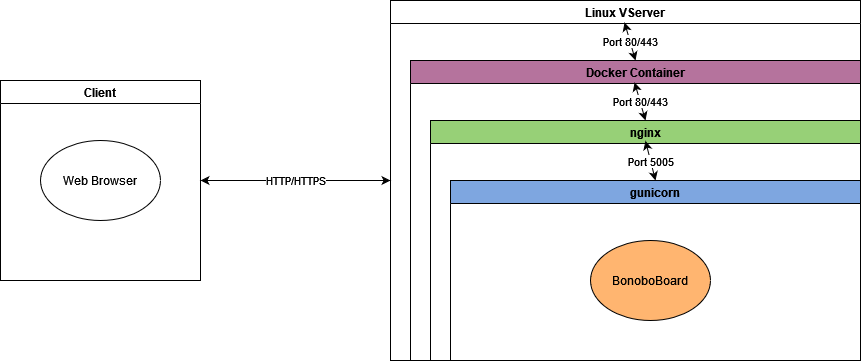
\includegraphics[width=\textwidth]{Serverstruktur}
	\caption{Serverstruktur BonoboBoard}
	\label{img:Serverstruktur}
\end{figure}

Die Anwendung selbst folgt dem "`Model-View-Presenter"' Schema (MVP), welches aus dem "`Model-View-Controller"' Schema (MVC) hervorgegangen ist. %TODO hervorgeht?
Dieses wird vom Django Framework vorgegeben. 

\begin{figure}[H]
\begin{center}
	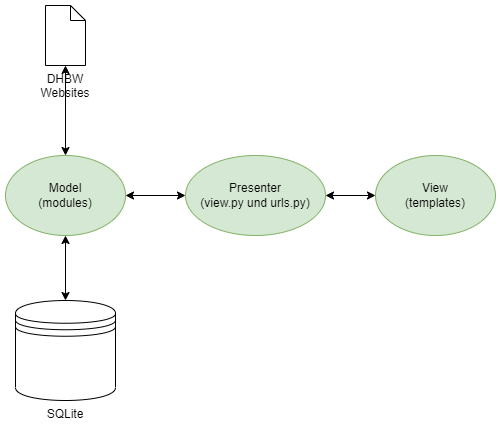
\includegraphics[width=0.6\textwidth]{MVP}
	\caption{Model-View-Presenter Schema des BonoboBoards}
	\label{img:MVP}
\end{center}
\end{figure}


Abbildung \ref{img:MVP} zeigt das Model-View-Presenter Schema des BonoboBoards und, wie die einzelnen Komponenten miteinander agieren. Diese Komponenten werden im Folgenden näher beschriebebn.

\paragraph{Model}
Das Model beinhaltet die Daten, welche angezeigt werden sollen. Es stellt die Logik der View dar und wird vom Presenter gesteuert. Das Modell ist die Schnittstelle zu den Scrapern, die die Daten von den jeweiligen Websites beziehen und zu einer SQLite Datenbank, welche aufbereitete Daten hält. Das Model wird durch Objekte in \texttt{modules/dhbw} realisiert, über die es mit der Datenbasis interagieren kann.

\paragraph{View}
Die View ist für die Darstellung der Website gegenüber den Nutzer*innen verantwortlich. Sie hat keinen Zugriff auf das Model oder den Presenter, sondern kümmert sich lediglich darum, wie die bereitgestellten Informationen angezeigt werden und nimmt Nutzereingaben für den Presenter entgegen. In Django werden die Views in Form von HTML-Templates realisiert. Dabei handelt es sich um HTML-Dateien, bei denen variable Informationen mittels spezieller Tags gekennzeichnet werden.

\paragraph{Presenter}
Der Presenter ist das Bindeglied zwischen View und Model. Er steuert, welche Elemente aus dem Modell an die View übergeben werden, damit diese angezeigt werden können. Der Presenter ist für die Verarbeitung von Nutzereingaben zuständig. Diese Funktion wird in Django von zwei Modulen übernommen: \texttt{urls.py} und den \texttt{urls.py} Modulen. \texttt{urls.py} ist für die Weiterleitung von Nutzeranfragen an die entsprechende Funktion in \texttt{view.py} zuständig, während \texttt{views.py} die Anfrage entgegennimmt und ein Sprechendes HTML-Template mit Informationen befüllt.


\section{Zusammenfassung}
Bei dem BonoboBoard handelt es sich um eine Client-Server-Anwendung, die ein Framework zur Grundlage hat, dass weite Teile der Architektur vorgibt. Das verwendete Framework Django folgt dem Model-View-Presenter Schema und wird verwendet, um Informationen aus einer Datenbank oder - mittels Scrapern - von Websites zu beziehen und anzuzeigen. %TODO der Gedankenstrich richtig platziert? -> - oder mittels Scrapern -


		%------------------------------------------------------------
		%-----  -----  ------ End actual content ------  -----  -----
		%------------------------------------------------------------
\end{document}